\documentclass[a4paper,12pt]{article}

\usepackage{cmap}					% поиск в PDF
\usepackage[T2A]{fontenc}			% кодировка
\usepackage[utf8]{inputenc}			% кодировка исходного текста
\usepackage[english,russian]{babel}	% локализация и переносы

%%% Страница
\usepackage{extsizes} % Возможность сделать 14-й шрифт
\usepackage{geometry} % Простой способ задавать поля
	\geometry{top=20mm}
	\geometry{bottom=20mm}
	\geometry{left=18mm}
	\geometry{right=18mm}
\usepackage{pdflscape}
\usepackage{afterpage}
\usepackage{rotating}
	
\usepackage{listings} %Листинг

%Таблица
\usepackage{tabularx}
\usepackage{multirow} % Слияние строк в таблице
\usepackage{graphicx}
\newcolumntype{C}{>{\centering\arraybackslash}X}
\newcolumntype{W}[1]{>{\centering\arraybackslash\hspace{0pt}}m{#1}}

\usepackage{array}
\renewcommand{\arraystretch}{1.2}

\newcolumntype{?}{!{\vrule width 2pt}}
\makeatletter
\def\hlinewd#1{%
\noalign{\ifnum0=`}\fi\hrule \@height #1 %
\futurelet\reserved@a\@xhline}
\makeatother

%Карты Карно
\usepackage{tikz}
\newcommand{\boundellipse}[3]% center, xdim, ydim
{(#1) ellipse (#2 and #3)
}
\usepackage{subcaption}

%Временная диаграмма
\usepackage{verbatim}
\usepackage{tikz-timing}

%Логические схемы
\usetikzlibrary{circuits.logic.IEC}
\usetikzlibrary{positioning}

\begin{document} % Конец преамбулы, начало текста.

%%% Титульный лист
\thispagestyle{empty}
\begin{center}	
	\textbf{НАЦИОНАЛЬНЫЙ ИССЛЕДОВАТЕЛЬСКИЙ ЯДЕРНЫЙ УНИВЕРСИТЕТ \\<<МИФИ>>}
\end{center}
\vspace{10ex}
\begin{center}
	\textbf{Лабораторная работа №~4}
	\vspace{1ex}

	по дисциплине <<Схемотехника ЭВМ>>
	\vspace{1ex}

	\textbf{<<Синхронные счетчики>>}
\end{center}
\vspace{8cm}
\begin{flushright}
	\noindent
	Работу выполнил:\\
	студент группы xxx\\
	Сайфуллина З.Р.\\
	\vspace{3ex}
	Преподаватель:\\
	Новиков~Г.Г.\\
	Ядыкин~И.М.\\
\end{flushright}
\begin{center}
	\vfill
	Москва 2016
\end{center}

\newpage
\textbf{Цель:} овладеть методом синтеза синхронных счетчиков; приобрести практические навыки отработки проектируемых схем как моделированием с использованием САПР, так и макетированием на универсальном лабораторном стенде.
\vspace{2ex}

\textbf{Задание:} Спроектировать трeхразрядный двоично-десятичный счетчик по данным:
\begin{table}[h!]
	\centering
		\begin{tabularx}{\textwidth}{|C|C|}
				\hline \textbf{Двоично-десятичный код} & \textbf{Десятичные номера двоичных наборов	последовательных десятичных цифр в данном двоично-десятичном коде} \\
				\hline	4621 	&	0, 1, 2, 3, 8, 9, 4, 5, 6, 7	\\
				\hline
		\end{tabularx}
\end{table}

\vspace{2ex}

\textbf{Требуется:}
\begin{enumerate}
\item{На основе матрицы переходов составить таблицу истинности функций возбуждения триггеров (DV и JK) счетчика;}
\item{Построить схемы двух разрядов (на DV и JK триггерах) двоично-десятичного счетчика с цепями переноса;}
\item{Описать счетчик на VHDL;}
\item{Построить схему соединения созданных счетчиков;}
\item{Разработать схему исследования спроектированных счетчиков с использованием макроэлементов стенда и осциллографа;}
\item{Получить результаты экспериментальных исследований.}
\end{enumerate}

\begin{figure}[!htb]\centering
\caption{Эталонная диаграмма Вейча}
\begin{tikzpicture}
	\draw (0,0) grid (4,4);
	\node at (3.5,.5){0};%0
	\node at (2.5,.5){1};%1
	\node at (3.5,1.5){2};%2
	\node at (2.5,1.5){3};%3
	\node at (.5,.5){4};%4
	\node at (1.5,.5){5};%5
	\node at (.5,1.5){6};%6
	\node at (1.5,1.5){7};%7
	\node at (3.5,3.5){8};%8
	\node at (2.5,3.5){9};%9
	\node at (3.5,2.5){10};%10
	\node at (2.5,2.5){11};%11
	\node at (.5,3.5){12};%12
	\node at (1.5,3.5){13};%13
	\node at (.5,2.5){14};%14
	\node at (1.5,2.5){15};%15
	\draw (-0.3,4) --node[midway, left]{Q$_3$} (-0.3,2);
	\draw (0,4.3) --node[midway, above]{Q$_2$} (2,4.3);
	\draw (4.3,1) --node[midway, right]{Q$_1$} (4.3,3);
	\draw (1,-0.3) --node[midway, below]{Q$_0$} (3,-0.3);
\end{tikzpicture}
\end{figure}

%DV триггер
\newpage
Напишем таблицу состояний и матрицу переходов DV-триггера:
\begin{table}[!h]
	\begin{minipage}{.5\linewidth}
		\caption{Таблица состояний DV-триггера}
			\begin{tabularx}{.9\textwidth}{|C|C?C|}
					\hline \textbf{D} & \textbf{V} & \textbf{Q(t+1)} \\
					\hline	0	&	0	&	Q(t)	\\
					\hline	0	&	1	&	0	\\
					\hline	1	&	0	&	Q(t)	\\
					\hline	1	&	1	&	1 \\
					\hline
			\end{tabularx}
	\end{minipage}
	\begin{minipage}{.5\linewidth}
		\caption{Матрица переходов DV-триггера}
		\centering
		\begin{tabularx}{0.9\textwidth}{|W{3cm}?C|C|}
				\hline \textbf{Q(t)$\to$Q(t+1)} & \textbf{D} & \textbf{V} \\
				\hline	0$\to$0	&	$a_1$	&	$\bar{a_1}b_1$	\\
				\hline	0$\to$1	&	1	&	1	\\
				\hline	1$\to$0	&	0	&	1	\\
				\hline	1$\to$1	&	$a_2$	&	$a_2b_2$	\\
				\hline
		\end{tabularx}
	\end{minipage}
\end{table}
\begin{table}[h!]
	\caption{Таблица переходов и функций возбуждения DV-триггеров счетчика}
	\centering
	\begin{tabularx}{\textwidth}{|W{1.5cm}|W{1.5cm}?C|C|C|C?C|C|C|C?W{0.4cm}|W{0.7cm}?W{0.4cm}|W{0.7cm}?W{0.4cm}|W{0.7cm}?C|C|}
		\hline
		\textbf{10-тичная цифра} & \textbf{№ набора} & \textbf{Q$_3$} & \textbf{Q$_2$} & \textbf{Q$_1$} & \textbf{Q$_0$} & \textbf{Q$_3$} & \textbf{Q$_2$} & \textbf{Q$_1$} & \textbf{Q$_0$} & \textbf{D$_3$} & \textbf{V$_3$} & \textbf{D$_2$} & \textbf{V$_2$} & \textbf{D$_1$} & \textbf{V$_1$} & \textbf{D$_0$} & \textbf{V$_0$} \\ \hline
		0 & 0 &		0 & 0 & 0 & 0 &		0 & 0 & 0 & 1 &		$a_0$ &	$\bar{a_0}b_0$ &		$a_0$ &	$\bar{a_0}b_0$ &		$a_0$ &	$\bar{a_0}b_0$ &		1 & 1	\\ \hline
		1 & 1 &		0 & 0 & 0 & 1 &		0 & 0 & 1 & 0 &		$a_1$ &	$\bar{a_1}b_1$ &		$a_1$ &	$\bar{a_1}b_1$ &		1 &	1 &		0 & 1	\\ \hline
		2 & 2 &		0 & 0 & 1 & 0 &		0 & 0 & 1 & 1 &		$a_2$ &	$\bar{a_2}b_2$ &		$a_2$ &	$\bar{a_2}b_2$ &		$a_2$ &	$a_2b_2$ &		1 & 1	\\ \hline
		3 & 3 &		0 & 0 & 1 & 1 &		1 & 0 & 0 & 0 &		1 &	1 &		$a_3$ &	$\bar{a_3}b_3$ &		0 &	1 &		0 & 1	\\ \hline
		4 & 8 &		1 & 0 & 0 & 0 &		1 & 0 & 0 & 1 &		$a_8$ &	$a_8b_8$ &		$a_8$ &	$\bar{a_8}b_8$ &		$a_8$ &	$\bar{a_8}b_8$ &		1 & 1	\\ \hline
		5 & 9 &		1 & 0 & 0 & 1 &		0 & 1 & 0 & 0 &		0 &	1 &		1 &	1 &		$a_9$ &	$\bar{a_9}b_9$ &		0 & 1	\\ \hline
		6 & 4 &		0 & 1 & 0 & 0 &		0 & 1 & 0 & 1 &		$a_4$ &	$\bar{a_4}b_4$ &		$a_4$ &	$a_4b_4$ &		$a_4$ &	$a_4b_4$ &		1 & 1	\\ \hline
		7 & 5 &		0 & 1 & 0 & 1 &		0 & 1 & 1 & 0 &		$a_5$ &	$\bar{a_5}b_5$ &		$a_5$ &	$a_5b_5$ &		1 &	1 &		0 & 1	\\ \hline
		8 & 6 &		0 & 1 & 1 & 0 &		0 & 1 & 1 & 1 &		$a_6$ &	$\bar{a_6}b_6$ &		$a_6$ &	$a_6b_6$ &		$a_6$ &	$a_6b_6$ &		1 & 1	\\ \hline
		9 & 7 &		0 & 1 & 1 & 1 &		0 & 0 & 0 & 0 &		$a_7$ &	$\bar{a_7}b_7$ &		0 &	1 &		0 &	1 &		0 & 1	\\ \hline
	\end{tabularx}
\end{table}

\newpage
Найдем минимальную ДНФ для функций D$_0$ и V$_0$:
\captionsetup[subfigure]{labelformat=empty}
\begin{figure}[!htb]\centering
\subcaptionbox{Диаграмма D$_0$}{
	\begin{tikzpicture}
	\draw (0,0) grid (4,4);
	\node at (3.5,.5){1};%0
	\node at (2.5,.5){0};%1
	\node at (3.5,1.5){1};%2
	\node at (2.5,1.5){0};%3
	\node at (3.5,3.5){1};%8
	\node at (2.5,3.5){0};%9
	\node at (.5,.5){1};%4
	\node at (1.5,.5){0};%5
	\node at (.5,1.5){1};%6
	\node at (1.5,1.5){0};%7
	\node at (3.5,2.5){x};%10
	\node at (2.5,2.5){x};%11
	\node at (.5,3.5){x};%12
	\node at (1.5,3.5){x};%13
	\node at (.5,2.5){x};%14
	\node at (1.5,2.5){x};%15
	\draw \boundellipse{0,2}{0.9}{1.9};
	\draw \boundellipse{4,2}{0.9}{1.9};
	\fill[white] (-.1,4.1) rectangle (-1,-.1);
	\fill[white] (4.1,-.1) rectangle (5,4);
	\draw (-0.3,4) --node[midway, left]{Q$_3$} (-0.3,2);
	\draw (0,4.3) --node[midway, above]{Q$_2$} (2,4.3);
	\draw (4.3,1) --node[midway, right]{Q$_1$} (4.3,3);
	\draw (1,-0.3) --node[midway, below]{Q$_0$} (3,-0.3);
	\end{tikzpicture}}\quad
\subcaptionbox{Диаграмма V$_0$}{
	\begin{tikzpicture}
	\draw (0,0) grid (4,4);
	\node at (3.5,.5){1};%0
	\node at (2.5,.5){1};%1
	\node at (3.5,1.5){1};%2
	\node at (2.5,1.5){1};%3
	\node at (3.5,3.5){1};%8
	\node at (2.5,3.5){1};%9
	\node at (.5,.5){1};%4
	\node at (1.5,.5){1};%5
	\node at (.5,1.5){1};%6
	\node at (1.5,1.5){1};%7
	\node at (3.5,2.5){x};%10
	\node at (2.5,2.5){x};%11
	\node at (.5,3.5){x};%12
	\node at (1.5,3.5){x};%13
	\node at (.5,2.5){x};%14
	\node at (1.5,2.5){x};%15	
	\draw (-0.3,4) --node[midway, left]{Q$_3$} (-0.3,2);
	\draw (0,4.3) --node[midway, above]{Q$_2$} (2,4.3);
	\draw (4.3,1) --node[midway, right]{Q$_1$} (4.3,3);
	\draw (1,-0.3) --node[midway, below]{Q$_0$} (3,-0.3);
	\draw \boundellipse{2,2}{1.9}{1.9};
	\end{tikzpicture}}
\end{figure}

Выпишем минимальные ДНФ функций D$_0$ и V$_0$:
\[
	D_0 =  \bar{Q}_0
\]
\[
	V_0 = 1
\]

Найдем минимальную ДНФ для функций D$_1$ и V$_1$:
\captionsetup[subfigure]{labelformat=empty}
\begin{figure}[!htb]\centering
\subcaptionbox{Диаграмма D$_1$}{
	\begin{tikzpicture}
	\draw (0,0) grid (4,4);
	\node at (3.5,.5){$a_0$};%0
	\node at (2.5,.5){1};%1
	\node at (3.5,1.5){$a_2$};%2
	\node at (2.5,1.5){0};%3
	\node at (3.5,3.5){$a_8$};%8
	\node at (2.5,3.5){$a_9$};%9
	\node at (.5,.5){$a_4$};%4
	\node at (1.5,.5){1};%5
	\node at (.5,1.5){$a_6$};%6
	\node at (1.5,1.5){0};%7
	\node at (3.5,2.5){x};%10
	\node at (2.5,2.5){x};%11
	\node at (.5,3.5){x};%12
	\node at (1.5,3.5){x};%13
	\node at (.5,2.5){x};%14
	\node at (1.5,2.5){x};%15
	\draw \boundellipse{2,0}{1.9}{0.9};
	\draw \boundellipse{2,4}{1.9}{0.9};
	\fill[white] (-.1,4.1) rectangle (4,5);
	\fill[white] (-.1,-.1) rectangle (4,-1);
	\draw (-0.3,4) --node[midway, left]{Q$_3$} (-0.3,2);
	\draw (0,4.3) --node[midway, above]{Q$_2$} (2,4.3);
	\draw (4.3,1) --node[midway, right]{Q$_1$} (4.3,3);
	\draw (1,-0.3) --node[midway, below]{Q$_0$} (3,-0.3);
	\end{tikzpicture}}\quad
\subcaptionbox{Диаграмма V$_1$}{
	\begin{tikzpicture}
	\draw (0,0) grid (4,4);
	\node at (3.5,.5){$\bar{a_0}b_0$};%0
	\node at (2.5,.5){1};%1
	\node at (3.5,1.5){$a_2b_2$};%2
	\node at (2.5,1.5){1};%3
	\node at (3.5,3.5){$\bar{a_8}b_8$};%8
	\node at (2.5,3.5){$\bar{a_9}b_9$};%9
	\node at (.5,.5){$\bar{a_4}b_4$};%4
	\node at (1.5,.5){1};%5
	\node at (.5,1.5){$a_6b_6$};%6
	\node at (1.5,1.5){1};%7
	\node at (3.5,2.5){x};%10
	\node at (2.5,2.5){x};%11
	\node at (.5,3.5){x};%12
	\node at (1.5,3.5){x};%13
	\node at (.5,2.5){x};%14
	\node at (1.5,2.5){x};%15
	\draw (-0.3,4) --node[midway, left]{Q$_3$} (-0.3,2);
	\draw (0,4.3) --node[midway, above]{Q$_2$} (2,4.3);
	\draw (4.3,1) --node[midway, right]{Q$_1$} (4.3,3);
	\draw (1,-0.3) --node[midway, below]{Q$_0$} (3,-0.3);
	\draw \boundellipse{2,1}{0.9}{0.9};
	\end{tikzpicture}}
\end{figure}

Выпишем минимальные ДНФ функций D$_1$ и V$_1$:
\[
	D_1 =  \bar{Q}_1
\]
\[
	V_1 = \bar{Q_3}Q_0
\]

\newpage
Найдем минимальную ДНФ для функций D$_2$ и V$_2$:
\captionsetup[subfigure]{labelformat=empty}
\begin{figure}[!htb]\centering
\subcaptionbox{Диаграмма D$_2$}{
	\begin{tikzpicture}
	\draw (0,0) grid (4,4);
	\node at (3.5,.5){$a_0$};%0
	\node at (2.5,.5){$a_1$};%1
	\node at (3.5,1.5){$a_2$};%2
	\node at (2.5,1.5){$a_3$};%3
	\node at (3.5,3.5){$a_8$};%8
	\node at (2.5,3.5){1};%9
	\node at (.5,.5){$a_4$};%4
	\node at (1.5,.5){$a_5$};%5
	\node at (.5,1.5){$a_6$};%6
	\node at (1.5,1.5){0};%7
	\node at (3.5,2.5){x};%10
	\node at (2.5,2.5){x};%11
	\node at (.5,3.5){x};%12
	\node at (1.5,3.5){x};%13
	\node at (.5,2.5){x};%14
	\node at (1.5,2.5){x};%15
	\draw (-0.3,4) --node[midway, left]{Q$_3$} (-0.3,2);
	\draw (0,4.3) --node[midway, above]{Q$_2$} (2,4.3);
	\draw (4.3,1) --node[midway, right]{Q$_1$} (4.3,3);
	\draw (1,-0.3) --node[midway, below]{Q$_0$} (3,-0.3);
	\draw \boundellipse{2,3}{1.9}{0.9};
	\draw \boundellipse{3.5,2}{0.4}{1.9};
	\end{tikzpicture}}\quad
\subcaptionbox{Диаграмма V$_2$}{
	\begin{tikzpicture}
	\draw (0,0) grid (4,4);
	\node at (3.5,.5){$\bar{a_0}b_0$};%0
	\node at (2.5,.5){$\bar{a_1}b_1$};%1
	\node at (3.5,1.5){$\bar{a_2}b_2$};%2
	\node at (2.5,1.5){$\bar{a_3}b_3$};%3
	\node at (3.5,3.5){$\bar{a_8}b_8$};%8
	\node at (2.5,3.5){1};%9
	\node at (.5,.5){$a_4b_4$};%4
	\node at (1.5,.5){$a_5b_5$};%5
	\node at (.5,1.5){$a_6b_6$};%6
	\node at (1.5,1.5){1};%7
	\node at (3.5,2.5){x};%10
	\node at (2.5,2.5){x};%11
	\node at (.5,3.5){x};%12
	\node at (1.5,3.5){x};%13
	\node at (.5,2.5){x};%14
	\node at (1.5,2.5){x};%15
	\draw (-0.3,4) --node[midway, left]{Q$_3$} (-0.3,2);
	\draw (0,4.3) --node[midway, above]{Q$_2$} (2,4.3);
	\draw (4.3,1) --node[midway, right]{Q$_1$} (4.3,3);
	\draw (1,-0.3) --node[midway, below]{Q$_0$} (3,-0.3);
	\draw \boundellipse{2,2}{0.9}{0.9};
	\draw \boundellipse{2.5,2}{0.4}{1.9};
	\end{tikzpicture}}
\end{figure}

Выпишем минимальные ДНФ функций D$_2$ и V$_2$:
\[
	D_2 =  Q_3 \vee \bar{Q}_2\bar{Q}_0
\]
\[
	V_2 = Q_1Q_0 \vee \bar{Q}_2Q_2
\]

Найдем минимальную ДНФ для функций D$_3$ и V$_3$:
\captionsetup[subfigure]{labelformat=empty}
\begin{figure}[!htb]\centering
\subcaptionbox{Диаграмма D$_3$}{
	\begin{tikzpicture}
	\draw (0,0) grid (4,4);
	\node at (3.5,.5){$a_0$};%0
	\node at (2.5,.5){$a_1$};%1
	\node at (3.5,1.5){$a_2$};%2
	\node at (2.5,1.5){1};%3
	\node at (3.5,3.5){$a_8$};%8
	\node at (2.5,3.5){0};%9
	\node at (.5,.5){$a_4$};%4
	\node at (1.5,.5){$a_5$};%5
	\node at (.5,1.5){$a_6$};%6
	\node at (1.5,1.5){$a_7$};%7
	\node at (3.5,2.5){x};%10
	\node at (2.5,2.5){x};%11
	\node at (.5,3.5){x};%12
	\node at (1.5,3.5){x};%13
	\node at (.5,2.5){x};%14
	\node at (1.5,2.5){x};%15
	\draw (-0.3,4) --node[midway, left]{Q$_3$} (-0.3,2);
	\draw (0,4.3) --node[midway, above]{Q$_2$} (2,4.3);
	\draw (4.3,1) --node[midway, right]{Q$_1$} (4.3,3);
	\draw (1,-0.3) --node[midway, below]{Q$_0$} (3,-0.3);
	\draw \boundellipse{2,2}{1.9}{0.9};
	\end{tikzpicture}}\quad
\subcaptionbox{Диаграмма V$_3$}{
	\begin{tikzpicture}
	\draw (0,0) grid (4,4);
	\node at (3.5,.5){$\bar{a_0}b_0$};%0
	\node at (2.5,.5){$\bar{a_1}b_1$};%1
	\node at (3.5,1.5){$\bar{a_2}b_2$};%2
	\node at (2.5,1.5){1};%3
	\node at (3.5,3.5){$a_8b_8$};%8
	\node at (2.5,3.5){1};%9
	\node at (.5,.5){$\bar{a_4}b_4$};%4
	\node at (1.5,.5){$\bar{a_5}b_5$};%5
	\node at (.5,1.5){$\bar{a_6}b_6$};%6
	\node at (1.5,1.5){$\bar{a_7}b_7$};%7
	\node at (3.5,2.5){x};%10
	\node at (2.5,2.5){x};%11
	\node at (.5,3.5){x};%12
	\node at (1.5,3.5){x};%13
	\node at (.5,2.5){x};%14
	\node at (1.5,2.5){x};%15
	\draw (-0.3,4) --node[midway, left]{Q$_3$} (-0.3,2);
	\draw (0,4.3) --node[midway, above]{Q$_2$} (2,4.3);
	\draw (4.3,1) --node[midway, right]{Q$_1$} (4.3,3);
	\draw (1,-0.3) --node[midway, below]{Q$_0$} (3,-0.3);
	\draw \boundellipse{2.5,2}{0.4}{1.9};
	\draw \boundellipse{2,0.5}{1.9}{0.4};
	\end{tikzpicture}}
\end{figure}

Выпишем минимальные ДНФ функций D$_3$ и V$_3$:
\[
	D_3 =  Q_1
\]
\[
	V_3 = \bar{Q}_3\bar{Q}_1 \vee \bar{Q}_2Q_0
\]

%JK триггер
\newpage
Напишем таблицу состояний и матрицу переходов JK-триггера:
\begin{table}[!htb]
	\begin{minipage}{.5\linewidth}
		\caption{Таблица состояний JK-триггера}
			\begin{tabularx}{.9\textwidth}{|C|C?C|}
					\hline \textbf{J} & \textbf{K} & \textbf{Q(t+1)} \\
					\hline	0	&	0	&	Q(t)	\\
					\hline	0	&	1	&	0	\\
					\hline	1	&	0	&	1	\\
					\hline	1	&	1	&	$\overline{Q(t)}$ \\
					\hline
			\end{tabularx}
	\end{minipage}
	\begin{minipage}{.5\linewidth}
		\caption{Матрица переходов JK-триггера}
		\centering
		\begin{tabularx}{0.9\textwidth}{|W{3cm}?C|C|}
				\hline \textbf{Q(t)$\to$Q(t+1)} & \textbf{J} & \textbf{K} \\
				\hline	0$\to$0	&	0	&	x	\\
				\hline	0$\to$1	&	1	&	x	\\
				\hline	1$\to$0	&	x	&	1	\\
				\hline	1$\to$1	&	x	&	0	\\
				\hline
		\end{tabularx}
	\end{minipage}
\end{table}
\begin{table}[!htb]
	\caption{Таблица переходов и функций возбуждения JK-триггеров счетчика}
	\centering
	\begin{tabularx}{\textwidth}{|W{1.5cm}|W{1.5cm}?C|C|C|C?C|C|C|C?C|C?C|C?C|C?C|C|}
	\hline
	\textbf{10-тичная цифра} & \textbf{№ набора} & \textbf{Q$_3$} & \textbf{Q$_2$} & \textbf{Q$_1$} & \textbf{Q$_0$} & \textbf{Q$_3$} & \textbf{Q$_2$} & \textbf{Q$_1$} & \textbf{Q$_0$} & \textbf{J$_3$} & \textbf{K$_3$} & \textbf{J$_2$} & \textbf{K$_2$} & \textbf{J$_1$} & \textbf{K$_1$} & \textbf{J$_0$} & \textbf{K$_0$} \\ \hline
	0 & 0 &		0 & 0 & 0 & 0 &		0 & 0 & 0 & 1 &		0 &	x &		0 &	x &		0 &	x &		1 & x	\\ \hline
	1 & 1 &		0 & 0 & 0 & 1 &		0 & 0 & 1 & 0 &		0 &	x &		0 &	x &		1 &	x &		x & 1	\\ \hline
	2 & 2 &		0 & 0 & 1 & 0 &		0 & 0 & 1 & 1 &		0 &	x &		0 &	x &		x &	0 &		1 & x	\\ \hline
	3 & 3 &		0 & 0 & 1 & 1 &		1 & 0 & 0 & 0 &		1 &	x &		0 &	x &		x &	1 &		x & 1	\\ \hline
	4 & 8 &		1 & 0 & 0 & 0 &		1 & 0 & 0 & 1 &		x &	0 &		0 &	x &		0 &	x &		1 & x	\\ \hline
	5 & 9 &		1 & 0 & 0 & 1 &		0 & 1 & 0 & 0 &		x &	1 &		1 &	x &		0 &	x &		x & 1	\\ \hline
	6 & 4 &		0 & 1 & 0 & 0 &		0 & 1 & 0 & 1 &		0 &	x &		x &	0 &		0 &	x &		1 & x	\\ \hline
	7 & 5 &		0 & 1 & 0 & 1 &		0 & 1 & 1 & 0 &		0 &	x &		x &	0 &		1 &	x &		x & 1	\\ \hline
	8 & 6 &		0 & 1 & 1 & 0 &		0 & 1 & 1 & 1 &		0 &	x &		x &	0 &		x &	0 &		1 & x	\\ \hline
	9 & 7 &		0 & 1 & 1 & 1 &		0 & 0 & 0 & 0 &		0 &	x &		x &	1 &		x &	1 &		x & 1	\\ \hline
	\end{tabularx}
\end{table}

Найдем минимальную ДНФ для функций J$_0$ и K$_0$:
\captionsetup[subfigure]{labelformat=empty}
\begin{figure}[!htb]\centering
\subcaptionbox{Диаграмма J$_0$}{
	\begin{tikzpicture}
	\draw (0,0) grid (4,4);
	\node at (3.5,.5){1};%0
	\node at (2.5,.5){1};%1
	\node at (3.5,1.5){1};%2
	\node at (2.5,1.5){1};%3
	\node at (.5,.5){1};%4
	\node at (1.5,.5){1};%5
	\node at (.5,1.5){1};%6
	\node at (1.5,1.5){1};%7
	\node at (3.5,3.5){1};%8
	\node at (2.5,3.5){1};%9
	\node at (3.5,2.5){x};%10
	\node at (2.5,2.5){x};%11
	\node at (.5,3.5){x};%12
	\node at (1.5,3.5){x};%13
	\node at (.5,2.5){x};%14
	\node at (1.5,2.5){x};%15
	\draw (-0.3,4) --node[midway, left]{Q$_3$} (-0.3,2);
	\draw (0,4.3) --node[midway, above]{Q$_2$} (2,4.3);
	\draw (4.3,1) --node[midway, right]{Q$_1$} (4.3,3);
	\draw (1,-0.3) --node[midway, below]{Q$_0$} (3,-0.3);
	\draw \boundellipse{2,2}{1.9}{1.9};
	\end{tikzpicture}}\quad
\subcaptionbox{Диаграмма K$_0$}{
	\begin{tikzpicture}
	\draw (0,0) grid (4,4);
	\node at (3.5,.5){1};%0
	\node at (2.5,.5){1};%1
	\node at (3.5,1.5){1};%2
	\node at (2.5,1.5){1};%3
	\node at (.5,.5){1};%4
	\node at (1.5,.5){1};%5
	\node at (.5,1.5){1};%6
	\node at (1.5,1.5){1};%7
	\node at (3.5,3.5){1};%8
	\node at (2.5,3.5){1};%9
	\node at (3.5,2.5){x};%10
	\node at (2.5,2.5){x};%11
	\node at (.5,3.5){x};%12
	\node at (1.5,3.5){x};%13
	\node at (.5,2.5){x};%14
	\node at (1.5,2.5){x};%15
	\draw (-0.3,4) --node[midway, left]{Q$_3$} (-0.3,2);
	\draw (0,4.3) --node[midway, above]{Q$_2$} (2,4.3);
	\draw (4.3,1) --node[midway, right]{Q$_1$} (4.3,3);
	\draw (1,-0.3) --node[midway, below]{Q$_0$} (3,-0.3);
	\draw \boundellipse{2,2}{1.9}{1.9};
	\end{tikzpicture}}
\end{figure}

Выпишем минимальные ДНФ функций J$_0$ и K$_0$:
\[
	J_0 =  1
\]
\[
	K_0 = 1
\]

\newpage
Найдем минимальную ДНФ для функций J$_1$ и K$_1$:
\captionsetup[subfigure]{labelformat=empty}
\begin{figure}[!htb]\centering
\subcaptionbox{Диаграмма J$_1$}{
	\begin{tikzpicture}
	\draw (0,0) grid (4,4);
	\node at (3.5,.5){0};%0
	\node at (2.5,.5){1};%1
	\node at (3.5,1.5){0};%2
	\node at (2.5,1.5){1};%3
	\node at (.5,.5){0};%4
	\node at (1.5,.5){1};%5
	\node at (.5,1.5){0};%6
	\node at (1.5,1.5){1};%7
	\node at (3.5,3.5){0};%8
	\node at (2.5,3.5){0};%9
	\node at (3.5,2.5){x};%10
	\node at (2.5,2.5){x};%11
	\node at (.5,3.5){x};%12
	\node at (1.5,3.5){x};%13
	\node at (.5,2.5){x};%14
	\node at (1.5,2.5){x};%15
	\draw (-0.3,4) --node[midway, left]{Q$_3$} (-0.3,2);
	\draw (0,4.3) --node[midway, above]{Q$_2$} (2,4.3);
	\draw (4.3,1) --node[midway, right]{Q$_1$} (4.3,3);
	\draw (1,-0.3) --node[midway, below]{Q$_0$} (3,-0.3);
	\draw \boundellipse{2,1}{0.9}{0.9};
	\end{tikzpicture}}\quad
\subcaptionbox{Диаграмма K$_1$}{
	\begin{tikzpicture}
	\draw (0,0) grid (4,4);
	\node at (3.5,.5){0};%0
	\node at (2.5,.5){1};%1
	\node at (3.5,1.5){0};%2
	\node at (2.5,1.5){1};%3
	\node at (.5,.5){0};%4
	\node at (1.5,.5){1};%5
	\node at (.5,1.5){0};%6
	\node at (1.5,1.5){1};%7
	\node at (3.5,3.5){0};%8
	\node at (2.5,3.5){1};%9
	\node at (3.5,2.5){x};%10
	\node at (2.5,2.5){x};%11
	\node at (.5,3.5){x};%12
	\node at (1.5,3.5){x};%13
	\node at (.5,2.5){x};%14
	\node at (1.5,2.5){x};%15
	\draw (-0.3,4) --node[midway, left]{Q$_3$} (-0.3,2);
	\draw (0,4.3) --node[midway, above]{Q$_2$} (2,4.3);
	\draw (4.3,1) --node[midway, right]{Q$_1$} (4.3,3);
	\draw (1,-0.3) --node[midway, below]{Q$_0$} (3,-0.3);
	\draw \boundellipse{2,2}{0.9}{1.9};
	\end{tikzpicture}}
\end{figure}

Выпишем минимальные ДНФ функций J$_1$ и K$_1$:
\[
	J_1 =  \bar{Q}_3Q_0
\]
\[
	K_1 = Q_0
\]

Найдем минимальную ДНФ для функций J$_2$ и K$_2$:
\captionsetup[subfigure]{labelformat=empty}
\begin{figure}[!htb]\centering
\subcaptionbox{Диаграмма J$_2$}{
	\begin{tikzpicture}
	\draw (0,0) grid (4,4);
	\node at (3.5,.5){0};%0
	\node at (2.5,.5){0};%1
	\node at (3.5,1.5){0};%2
	\node at (2.5,1.5){0};%3
	\node at (.5,.5){0};%4
	\node at (1.5,.5){0};%5
	\node at (.5,1.5){0};%6
	\node at (1.5,1.5){0};%7
	\node at (3.5,3.5){0};%8
	\node at (2.5,3.5){1};%9
	\node at (3.5,2.5){x};%10
	\node at (2.5,2.5){x};%11
	\node at (.5,3.5){x};%12
	\node at (1.5,3.5){x};%13
	\node at (.5,2.5){x};%14
	\node at (1.5,2.5){x};%15
	\draw (-0.3,4) --node[midway, left]{Q$_3$} (-0.3,2);
	\draw (0,4.3) --node[midway, above]{Q$_2$} (2,4.3);
	\draw (4.3,1) --node[midway, right]{Q$_1$} (4.3,3);
	\draw (1,-0.3) --node[midway, below]{Q$_0$} (3,-0.3);
	\draw \boundellipse{2,3}{0.9}{0.9};
	\end{tikzpicture}}\quad
\subcaptionbox{Диаграмма K$_2$}{
	\begin{tikzpicture}
	\draw (0,0) grid (4,4);
	\node at (3.5,.5){0};%0
	\node at (2.5,.5){0};%1
	\node at (3.5,1.5){0};%2
	\node at (2.5,1.5){1};%3
	\node at (.5,.5){0};%4
	\node at (1.5,.5){0};%5
	\node at (.5,1.5){0};%6
	\node at (1.5,1.5){1};%7
	\node at (3.5,3.5){0};%8
	\node at (2.5,3.5){0};%9
	\node at (3.5,2.5){x};%10
	\node at (2.5,2.5){x};%11
	\node at (.5,3.5){x};%12
	\node at (1.5,3.5){x};%13
	\node at (.5,2.5){x};%14
	\node at (1.5,2.5){x};%15
	\draw (-0.3,4) --node[midway, left]{Q$_3$} (-0.3,2);
	\draw (0,4.3) --node[midway, above]{Q$_2$} (2,4.3);
	\draw (4.3,1) --node[midway, right]{Q$_1$} (4.3,3);
	\draw (1,-0.3) --node[midway, below]{Q$_0$} (3,-0.3);
	\draw \boundellipse{2,2}{0.9}{0.9};
	\end{tikzpicture}}
\end{figure}

Выпишем минимальные ДНФ функций J$_2$ и K$_2$:
\[
	J_2 =  Q_3Q_0
\]
\[
	K_2 = Q_0Q_1
\]

\newpage
Найдем минимальную ДНФ для функций J$_3$ и K$_3$:
\captionsetup[subfigure]{labelformat=empty}
\begin{figure}[!htb]\centering
\subcaptionbox{Диаграмма J$_3$}{
	\begin{tikzpicture}
	\draw (0,0) grid (4,4);
	\node at (3.5,.5){0};%0
	\node at (2.5,.5){0};%1
	\node at (3.5,1.5){0};%2
	\node at (2.5,1.5){1};%3
	\node at (.5,.5){0};%4
	\node at (1.5,.5){0};%5
	\node at (.5,1.5){0};%6
	\node at (1.5,1.5){0};%7
	\node at (3.5,3.5){0};%8
	\node at (2.5,3.5){0};%9
	\node at (3.5,2.5){x};%10
	\node at (2.5,2.5){x};%11
	\node at (.5,3.5){x};%12
	\node at (1.5,3.5){x};%13
	\node at (.5,2.5){x};%14
	\node at (1.5,2.5){x};%15
	\draw (-0.3,4) --node[midway, left]{Q$_3$} (-0.3,2);
	\draw (0,4.3) --node[midway, above]{Q$_2$} (2,4.3);
	\draw (4.3,1) --node[midway, right]{Q$_1$} (4.3,3);
	\draw (1,-0.3) --node[midway, below]{Q$_0$} (3,-0.3);
	\draw \boundellipse{2.5,2}{0.4}{0.9};
	\end{tikzpicture}}\quad
\subcaptionbox{Диаграмма K$_3$}{
	\begin{tikzpicture}
	\draw (0,0) grid (4,4);
	\node at (3.5,.5){0};%0
	\node at (2.5,.5){1};%1
	\node at (3.5,1.5){0};%2
	\node at (2.5,1.5){1};%3
	\node at (.5,.5){0};%4
	\node at (1.5,.5){1};%5
	\node at (.5,1.5){0};%6
	\node at (1.5,1.5){1};%7
	\node at (3.5,3.5){0};%8
	\node at (2.5,3.5){1};%9
	\node at (3.5,2.5){x};%10
	\node at (2.5,2.5){x};%11
	\node at (.5,3.5){x};%12
	\node at (1.5,3.5){x};%13
	\node at (.5,2.5){x};%14
	\node at (1.5,2.5){x};%15
	\draw (-0.3,4) --node[midway, left]{Q$_3$} (-0.3,2);
	\draw (0,4.3) --node[midway, above]{Q$_2$} (2,4.3);
	\draw (4.3,1) --node[midway, right]{Q$_1$} (4.3,3);
	\draw (1,-0.3) --node[midway, below]{Q$_0$} (3,-0.3);
	\draw \boundellipse{2,2}{0.9}{1.9};
	\end{tikzpicture}}
\end{figure}

Выпишем минимальные ДНФ функций J$_3$ и K$_3$:
\[
	J_3 =  \bar{Q}_2Q_1Q_0
\]
\[
	K_3 = Q_0
\]

Организация связи между двоично-десятичными счетчиками
\[
	Q_3Q_2Q_1Q_0 = 0111
\]
\begin{figure}[!htb]\centering
\subcaptionbox{Диаграмма TC}{
	\begin{tikzpicture}
	\draw (0,0) grid (4,4);
	\node at (3.5,.5){0};%0
	\node at (2.5,.5){0};%1
	\node at (3.5,1.5){0};%2
	\node at (2.5,1.5){0};%3
	\node at (.5,.5){0};%4
	\node at (1.5,.5){0};%5
	\node at (.5,1.5){0};%6
	\node at (1.5,1.5){1};%7
	\node at (3.5,3.5){0};%8
	\node at (2.5,3.5){0};%9
	\node at (3.5,2.5){x};%10
	\node at (2.5,2.5){x};%11
	\node at (.5,3.5){x};%12
	\node at (1.5,3.5){x};%13
	\node at (.5,2.5){x};%14
	\node at (1.5,2.5){x};%15
	\draw (-0.3,4) --node[midway, left]{Q$_3$} (-0.3,2);
	\draw (0,4.3) --node[midway, above]{Q$_2$} (2,4.3);
	\draw (4.3,1) --node[midway, right]{Q$_1$} (4.3,3);
	\draw (1,-0.3) --node[midway, below]{Q$_0$} (3,-0.3);
	\draw \boundellipse{1.5,2}{0.4}{0.9};
	\end{tikzpicture}}
\end{figure}
\[
	TC = Q_2Q_1Q_0
\]

Входной сигнал переноса CEO для дальнейшего увеличения разрядности двоично-десятичных счетчиков:
\[
	COE = TC \& CE
\]

\newpage
\textbf{Описание комбинационной схемы на языке VHDL:}
\begin{lstlisting}[frame=single, language=VHDL, breaklines=true, tabsize=6]  % Code
	entity Lab4 is
	port (
	  CLR,C,CE: in BIT;
	  Q: buffer BIT_VECTOR (3 downto 0);
	  TC: buffer BIT;
	  CEO: out BIT
	);
	end Lab4;
	architecture Lab4_arch of Lab4 is
	begin
	  process (CLR,C)
	  begin
	    if CLR='1' then Q <= "0000";
	    elsif CE='0' then null;
	    elsif C'event and C='1' then
	      case Q is
	      when "0000" => Q <= "0001";
	      when "0001" => Q <= "0010";
	      when "0010" => Q <= "0011";
	      when "0011" => Q <= "1000";
	      when "1000" => Q <= "1001";
	      when "1001" => Q <= "0100";
	      when "0100" => Q <= "0101";
	      when "0101" => Q <= "0110";
	      when "0110" => Q <= "0111";
	      when "0111" => Q <= "0000";
	      when others => Q <= "0000";
	      end case;
	    end if;
	  end process;
	  TC <= Q(2) and Q(1) and Q(0) ;
	  CEO <= CE and TC ;
	end Lab4_arch;
\end{lstlisting}

\newpage
\begin{figure}[!htb]
	\caption{Схема двоично-десятичного считчика с асинхронным входом предварительной установки в 0, построенного на DV-триггерах.}
	\label{fig:dvcount}
	% Схему рисую в xilinx
	\centering
	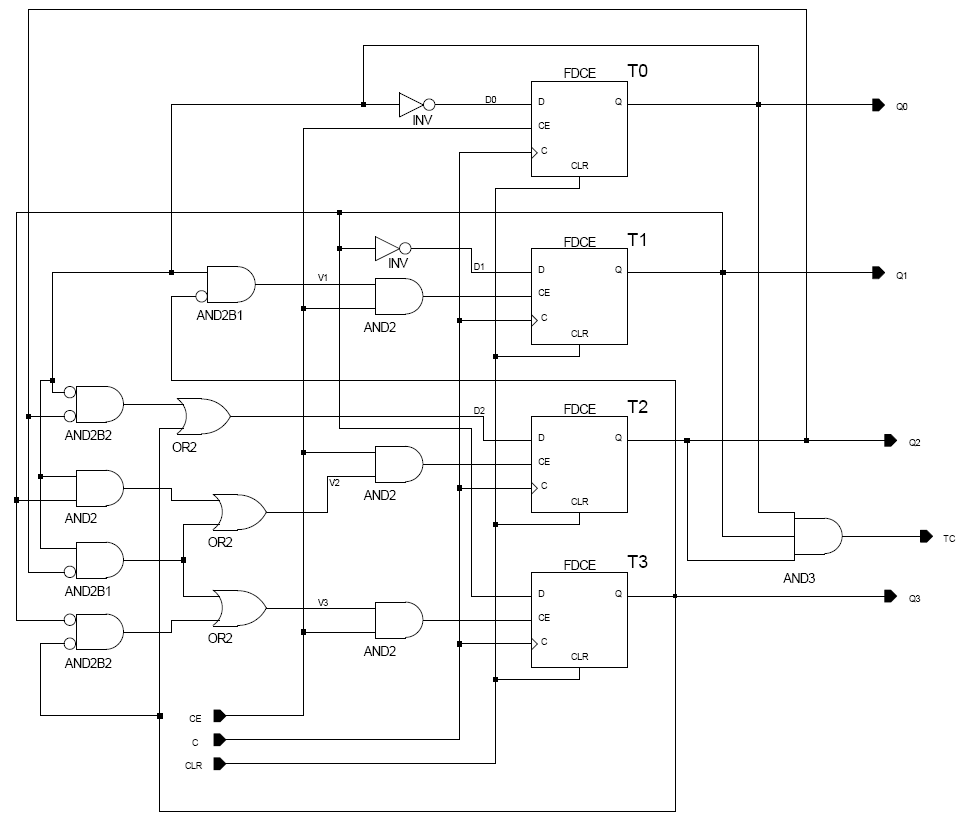
\includegraphics[scale=0.5]{lab4dv}
\end{figure}
% Временную диаграмму генерю в xilinx и подставляю задержки
\begin{figure}[!htb]	
	\caption{Временная диаграмма двоично-десятичного считчика с асинхронным входом предварительной установки в 0, построенного на DV-триггерах}
	\label{fig:dvtg}
	\centering
		\begin{tikztimingtable}[
			timing/slope=0,         % no slope
			timing/coldist=2pt,     % column distance
			xscale=0.56,yscale=1.5, % scale diagrams .5 
			semithick               % set line width
		]
				$C$		& 5L5H5L5H5L5H5L5H5L5H5L5H5L5H5L5H5L5H5L5H\\
				$D0$	& 5H10L10H10L10H10L10H10L10H10L5H \\
				$D1$	& 15H20L40H20L5H \\
				$D2$	& 5L10H10L10H30L10H10L10H5L \\
				$D3$	& 5H10L10H10L20H40L5H \\
				$D4$	& 5H10L10H10L10H50L5H \\
				$D5$	& 5L10H10L10H10L10H30L10H5L \\
				$D6$	& 25L10H50L10H5L \\
				$D7$	& 5L10H10L10H10L10H45L \\
				$D8$	& 15H10L10H10L30H20L5H \\
				$D9$	& 35L20H45L \\
				$Q0$	& 5L10H10L10H10L10H10L10H10L10H5L \\
				$Q1$	& 15L20H40L20H5L \\
				$Q2$	& 55L40H5L \\
				$Q3$	& 35L20H45L \\
				$TC$	& 85L10H5L \\
			\extracode
			\makeatletter
			\begin{pgfonlayer}{background}
				% Add background grid lines
				\begin{scope}[yellow,semitransparent,semithick]
					\foreach \x in {1,...,100}
						\draw (\x,1) -- (\x,-32);
				\end{scope}
				\begin{scope}[red,semitransparent,semithick]
					\foreach \x in {0,...,9}
						\draw (10*\x+5,1) -- (10*\x+5,-32);
				\end{scope}  
			\end{pgfonlayer}
		\end{tikztimingtable}
\end{figure}

\newpage
\begin{figure}[!htb]
	\caption{Схема двоично-десятичного считчика с асинхронным входом предварительной установки в 0, построенного на JK-триггерах.}
	\label{fig:jkcount}
	% Схему рисую в xilinx
	\centering
	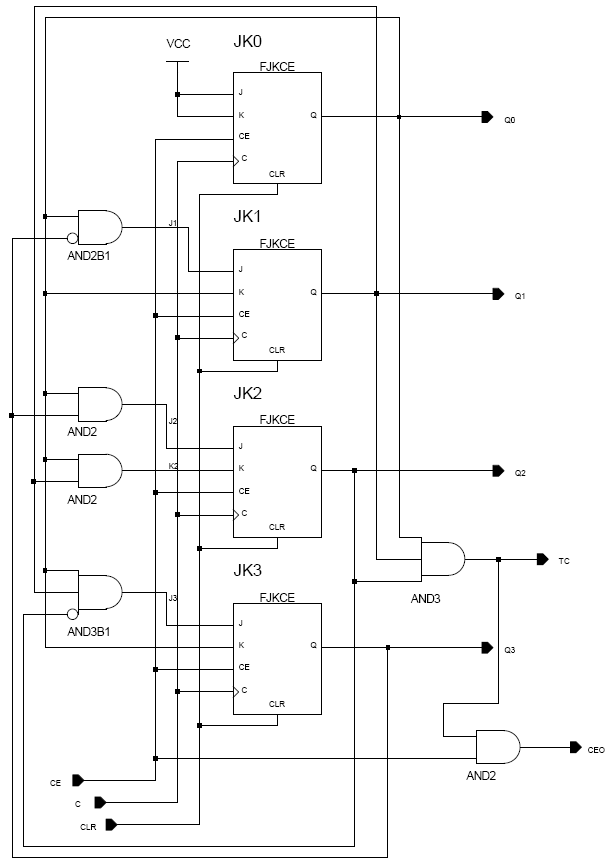
\includegraphics[scale=0.5]{lab4jk}
\end{figure}
% Временную диаграмму генерю в xilinx и подставляю задержки
\begin{figure}[!htb]	
	\caption{Временная диаграмма двоично-десятичного считчика с асинхронным входом предварительной установки в 0, построенного на JK-триггерах}
	\label{fig:jktg}
	\centering
		\begin{tikztimingtable}[
			timing/slope=0,         % no slope
			timing/coldist=2pt,     % column distance
			xscale=0.56,yscale=1.5, % scale diagrams .5 
			semithick               % set line width
		]
			$C$		& 5L5H5L5H5L5H5L5H5L5H5L5H5L5H5L5H5L5H5L5H\\
			$D0$	& 5L10H10L10H30L10H10L10H5L \\
			$D1$	& 45L10H45L \\
			$D2$	& 25L10H50L10H5L \\
			$D3$	& 25L10H65L \\
			$Q0$	& 5L10H10L10H10L10H10L10H10L10H5L \\
			$Q1$	& 15L20H40L20H5L \\
			$Q2$	& 55L40H5L \\
			$Q3$	& 35L20H45L \\
			$TC$	& 85L10H5L \\
			$CEO$	& 85L10H5L \\
			\extracode
			\makeatletter
			\begin{pgfonlayer}{background}
				% Add background grid lines
				\begin{scope}[yellow,semitransparent,semithick]
					\foreach \x in {1,...,100}
						\draw (\x,1) -- (\x,-20);
				\end{scope}
				\begin{scope}[red,semitransparent,semithick]
					\foreach \x in {0,...,9}
						\draw (10*\x+5,1) -- (10*\x+5,-20);
				\end{scope}
				%\begin{scope}[grey,semitransparent,semithick]
				%	\horlines{}
				%\end{scope}
			\end{pgfonlayer}
		\end{tikztimingtable}
\end{figure}


\newpage
\begin{landscape}
\begin{figure}[!htb]
	\caption{Схема подключения счетчиков}
	\label{fig:sch}
	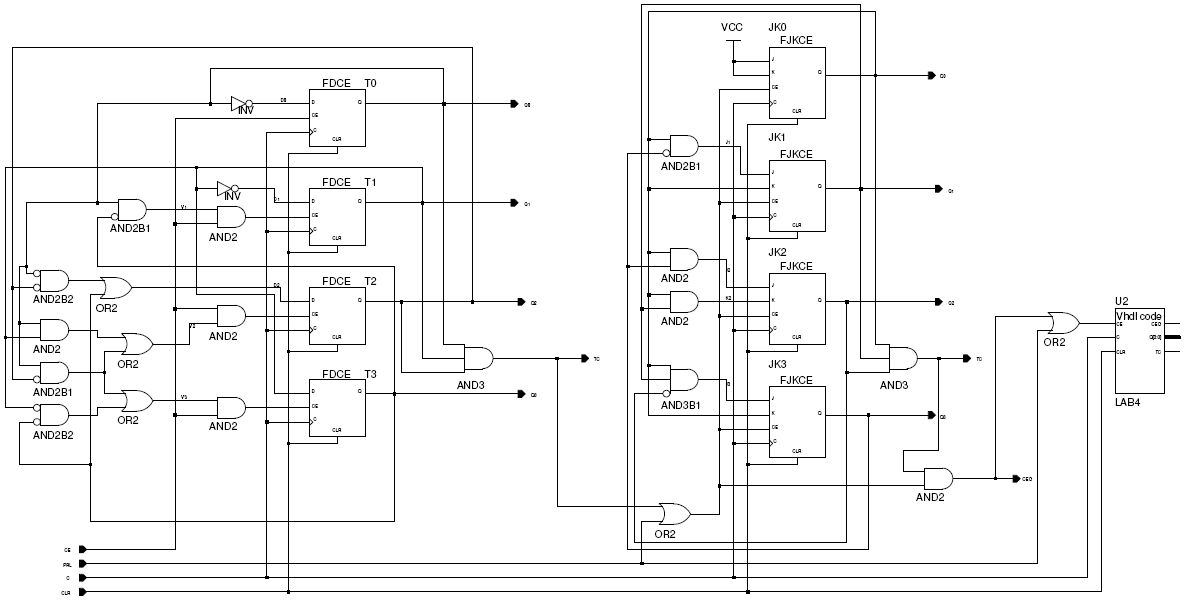
\includegraphics[scale=0.65]{lab4sch}
\end{figure}
\begin{figure}[!htb]
	\caption{Схема эксперимента}
	\label{fig:exp}
	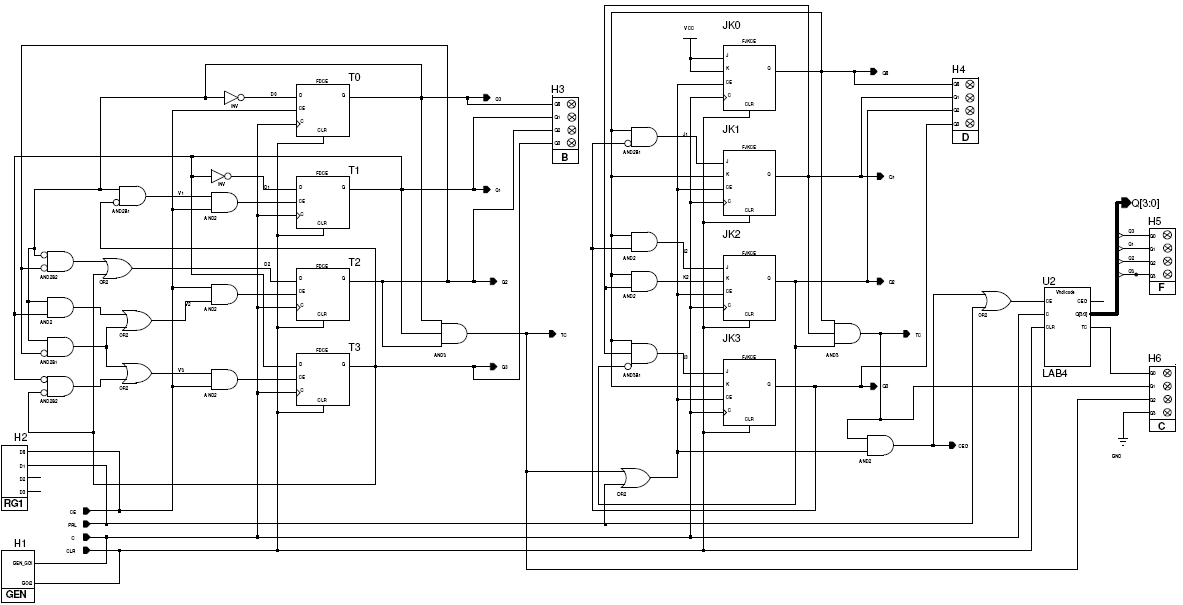
\includegraphics[scale=0.64]{lab4sexp}
\end{figure}
\end{landscape}
\end{document} % Конец текста.

